\documentclass[usenames,dvipsnames,aspectratio=1610]{beamer}

%\setbeamertemplate{nagivation symbols}{}
%%% Standard includes
\usepackage{amsthm, amssymb, amsmath, hyperref}
\usepackage{subfig,multicol}

\usepackage[T1]{fontenc}
\usepackage{lmodern}

\usetheme[sectionpage=none]{metropolis}
\setbeamertemplate{subsection in toc}[sections numbered]

%%% Graphics 
\usepackage{tikz}
\usetikzlibrary{shapes,arrows.meta,decorations.markings}
%\usepackage[all]{xy}
%\usepackage{graphicx}
%\usepackage{subcaption}


%%% Margins, formatting
%\usepackage{fullpage}
%\usepackage[margin=1in]{geometry}
\usepackage{setspace}
\usepackage{fancyhdr,lastpage}
%\usepackage{afterpage}
%\pagenumbering{gobble}
%\addtolength{\textwidth}{4cm}
%\addtolength{\hoffset}{-2cm}
%\addtolength{\textheight}{3.5cm}
%\addtolength{\voffset}{-2.5cm}
%\fancyhead{}
%\doublespacing
%\usepackage{enumitem} %%enumitem is incompatible with beamer
%\setitemize{noitemsep}
%\linespacing{1.1em}


%% Define the headers and footers for the first page, call it 'first'
%\fancypagestyle{first}{%
  %\renewcommand{\headrulewidth}{0pt}
%\fancyfoot[C]{\thepage~of~\pageref{LastPage}}
%\renewcommand{\footrulewidth}{0pt}}

%\usepackage{multicol}

%%% Bibliography
\usepackage[
backend=bibtex,
style=numeric,
block=space
]{biblatex}
\addbibresource{ref1.bib}
\renewbibmacro{in:}{}
\DeclareNameAlias{sortname}{first-last}

%%% Fonts
%\usepackage{helvet}
%\usepackage{anyfontsize,libertine}
%\usepackage{libertinust1math}
%\usepackage[T1]{fontenc}
%\usepackage{mathpazo}
%\usepackage{eulervm}
%\renewcommand{\familydefault}{\sfdefault}


% Quiet beamer complaints
\renewcommand\textbullet{\ensuremath{\bullet}}



%%% New commands

\newcommand{\Mdef}[2]{\newcommand{#1}{\relax \ifmmode #2 \else $#2$\fi}}

%% thereoms, prop, etc
%\newtheorem{theorem}{Theorem}
%\newtheorem{lemma}[theorem]{Lemma}
%\newtheorem{prop}[theorem]{Proposition}
%\newtheorem{definition}[theorem]{Definition}
%\newtheorem{corollary}[theorem]{Corollary}
%\newtheorem{example}[theorem]{Example}
%\newtheorem{remark}[theorem]{Remark}
%\newtheorem{conjecture}[theorem]{Conjecture}
%\newtheorem*{question}{Question}
%\newtheorem*{questions}{Questions}

%% operators
\DeclareMathOperator{\Hom}{Hom}
\DeclareMathOperator{\cok}{cok}
\DeclareMathOperator{\im}{im}
\DeclareMathOperator{\id}{id}

%% Letters
\Mdef{\SA}{\mathcal{A}}
\Mdef{\SAD}{\mathcal{A}_*}
\Mdef{\SAS}{\mathrm{Sq}}
\Mdef{\SAP}{\mathcal{P}}

\Mdef{\B}{B}
\Mdef{\F}{\mathbb{F}}
\Mdef{\M}{\mathcal{M}}
\Mdef{\N}{\mathbb{N}}
\Mdef{\R}{\mathbb{R}}
\Mdef{\Z}{\mathbb{Z}}
\Mdef{\Q}{\mathbb{Q}}
\Mdef{\vectk}{\mathrm{vect}_k}

\newcommand{\Fp}[1]{\mathbb{F}_{#1}}
\newcommand{\HPM}[1]{H_{#1}^{\mathrm{MP}}(f;\mathbb{F}_2)}


%% arrows
\newcommand{\ra}{\rightarrow}
\newcommand{\lra}{\longrightarrow}
\newcommand{\la}{\leftarrow}
\newcommand{\lla}{\longleftarrow}

%% symbols
\newcommand{\tensor}{\otimes}
\newcommand{\dsum}{\oplus}
\newcommand{\Dsum}{\bigoplus}
\newcommand{\susp}{\Sigma}



\tikzstyle{decision} = [diamond, draw, fill=blue!20, 
    text width=4.5em, text badly centered, node distance=3cm, inner sep=0pt]
\tikzstyle{block} = [rectangle, draw, fill=blue!20, 
    text width=5em, text centered, rounded corners, minimum height=4em]
\tikzstyle{wideblock} = [rectangle, draw, fill=blue!20, 
    text width=7em, text centered, rounded corners, minimum height=4em]
%\tikzstyle{line} = [draw, -latex']
\tikzstyle{line} = [draw, -Latex]
\tikzstyle{cloud} = [draw, ellipse,fill=red!20, node distance=3cm,
    minimum height=2em]
%%%%%%%%%%%%%%%%%%%%%%%%


\title{An Introduction to Topological Data Analysis}
\author{Matthew Zabka}
\date{Laber Labs \\ North Carolina State University}
\institute{Southwest Minnesota State University}

\begin{document}
\setbeamercolor{background canvas}{bg=white}
\begin{frame}[plain]
  \maketitle
\end{frame}

\metroset{block=fill}

\begin{frame}{Outline}
  \tableofcontents
\end{frame}

\section{Crash course in algebraic topology}
\begin{frame}
  \frametitle{Algebraic Topology}
  \begin{block}{What is algebraic topology?}
    Topology is a branch of mathematics which is good at extracting global
    qualitative features from complicated geometric structures. 
    
    Algebraic topology provides a set of {\em algebraic} descriptors to topological objects.
  \end{block}
  \pause

  \begin{block}{Questions and scope}
    Topological questions surround different notions of connectedness:
    connected components, loops, voids, etc.

    Two topological spaces are equivalent through the lens of topology if one
    can be {\em continuously} deformed to the other. 
  \end{block}
  \center{\fontsize{40}{40}\selectfont \textsf{A B C D}}
\end{frame}

\begin{frame}
  \frametitle{Algebraic Topology}
  \begin{block}{What is algebraic topology?}
    Topology is a branch of mathematics which is good at extracting global
    qualitative features from complicated geometric structures. 
    
    Algebraic topology provides a set of {\em algebraic} descriptors to topological objects.
  \end{block}

  \begin{block}{Questions and scope}
    Topological questions surround different notions of connectedness:
    connected components, loops, voids, etc.

    Two topological spaces are equivalent through the lens of topology if one
    can be {\em continuously} deformed to the other. 
  \end{block}
  \center{\fontsize{40}{40}\selectfont \textsf{ {\color{red} A} B C {\color{red} {D}}}}
\end{frame}

\begin{frame}{Invariants of topological spaces}
  \begin{itemize}
    \item Algebraic Topology assigns {\em invariants} to topological spaces.
      These take the form of groups, rings, fields, vector spaces, etc.
    \item Our computations will be over the field $\F_2$, so it suffices to record
      only the {\em dimensions} of vector spaces. 
    \item If two spaces are the same, then the invariants must be the same. 
      
      If the invariants are not the same, then the two spaces are not the same.
  \end{itemize}
\end{frame}

\section{Persistent Homology and examples}
\begin{frame}{Topological Data Analysis}
  \begin{alertblock}{Goal}
    {\bf Topological data analysis uses topology to summarize and study the
    `shape' of data.}
  \end{alertblock}
  \vspace{-0.1in}
  \pause
  Examples:
  \vspace{-0.1in}
  \begin{itemize}
  \begin{multicols}{2}
  \item motion tracking problems,
  \item analysis of brain arteries,
  \item analysis of social and spatial networks, including neuronal
    networks, Twitter, co-authorship,
  \item study of viral evolution,
  \item measurement of protein compressibility,
  \item analysis of phase transitions,
  \item financial crash analysis,
  \item piecewise constant signal analysis,
  \item study of cosmic web and its filamentary structure,
  \item identification of breast cancer subtypes,
  \item study of plant root systems,
  \item discrimination of EEG signals before and during epileptic seizures,
  \item steganalysis of images,
  \item sphere packings,
  \item population activity in the visual cortex,
  \item fMRI data
  \end{multicols}

  \end{itemize}
\end{frame}

\begin{frame}{Overview of TDA}
  Topological data analysis comes in a variety of flavors. 
  
  The two most popular methods in TDA are
  \begin{center}
    1. Persistent Homology \\
    2.  Mapper
  \end{center}
\end{frame}




\begin{frame}
  \frametitle{Simplicial Complexes}
  A {\em simplicial complex} is a combinatorial object, generalizing the notion of a graph. Each
  simplicial complex is built out of {\em simplices} of varying dimensions.

  \begin{center}
    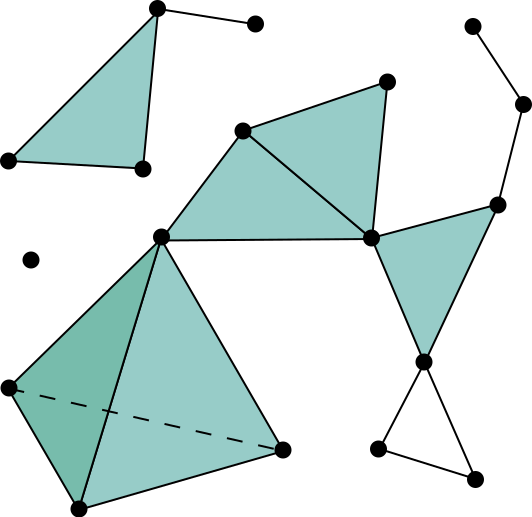
\includegraphics[scale=0.35]{images/Simplicial_complex_example.png}
  \end{center}
\end{frame}

\begin{frame}
  \frametitle{Betti numbers of simplicial complexes}
  \begin{align*}
    \beta_0 & =  \# \text{ of connected components}\\
    \beta_1 & =  \# \text{ of holes}\\
    \beta_2 & =  \# \text{ of voids}
  \end{align*}
  \begin{columns}
    \begin{column}{0.4\textwidth}
      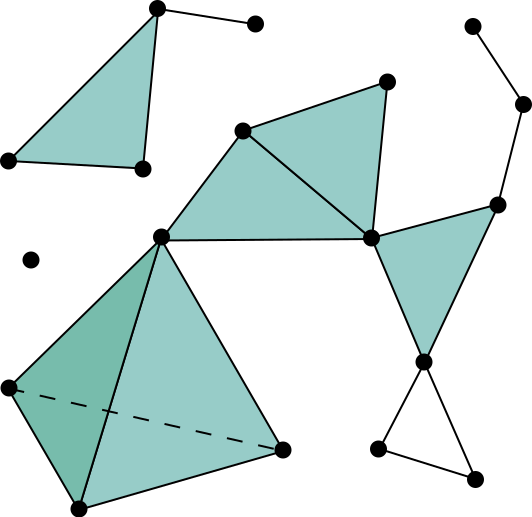
\includegraphics[height=45mm]{images/Simplicial_complex_example.png}
    \end{column}
    \begin{column}{0.2\textwidth}
      \begin{eqnarray*}
        \beta_0 & = & \visible<2>{3}\\
        \beta_1 & = & \visible<2>{1}\\
        \beta_2 & = & \visible<2>{1}
      \end{eqnarray*}
    \end{column}
  \end{columns}
  \bigskip
\end{frame}


\begin{frame} \frametitle{Homology of simplicial complexes}
  \begin{definition}
    Homology in degree $k$ is given by $k$-cycles modulo the $k$-boundaries.
  \end{definition}

\begin{center}
\definecolor{zzttqq}{rgb}{0.6,0.2,0}
\definecolor{qqqqff}{rgb}{0,0,1}
\begin{tikzpicture}[line cap=round,line join=round,x=1.0cm,y=1.0cm,scale=1.5]
% \draw[->,color=black] (-4.3,0) -- (7.5,0);
% \foreach \x in {-4,-3,-2,-1,1,2,3,4,5,6,7}
% \draw[shift={(\x,0)},color=black] (0pt,2pt) -- (0pt,-2pt) node[below] {\footnotesize $\x$};
% \draw[->,color=black] (0,-3.1) -- (0,6.3);
% \foreach \y in {-3,-2,-1,1,2,3,4,5,6}
% \draw[shift={(0,\y)},color=black] (2pt,0pt) -- (-2pt,0pt) node[left] {\footnotesize $\y$};
% \draw[color=black] (0pt,-10pt) node[right] {\footnotesize $0$};
% \clip(-4.3,-3.1) rectangle (7.5,6.3);
\fill[color=red,fill=red,fill opacity=0.2] (1,4.5) -- (2.1,5.3) -- (2.4,4.1) -- cycle;
\fill[color=red,fill=red,fill opacity=0.2] (1,4.5) -- (1,3) -- (2.4,4.1) -- cycle;
\fill[color=red,fill=red,fill opacity=0.2] (1,3) -- (1.8,2.2) -- (2.4,4.1) -- cycle;
\fill[color=red,fill=red,fill opacity=0.2] (1.8,2.2) -- (2.5,2.9) -- (2.4,4.1) -- cycle;
\fill[color=red,fill=red,fill opacity=0.2] (2.1,5.3) -- (3.7,4.9) -- (2.4,4.1) -- cycle;
\fill[color=red,fill=red,fill opacity=0.2] (3.7,4.9) -- (2.5,2.9) -- (2.4,4.1) -- cycle;
\fill[color=red,fill=red,fill opacity=0.2] (1.8,2.2) -- (3.1,2.2) -- (2.5,2.9) -- cycle;
\fill[color=red,fill=red,fill opacity=0.2] (3.1,2.2) -- (4,3) -- (5,2.3) -- cycle;
\fill[color=red,fill=red,fill opacity=0.2] (4,3) -- (4.8,3.2) -- (5,2.3) -- cycle;
\fill[color=red,fill=red,fill opacity=0.2] (5.5,4.7) -- (6.2,5.2) -- (6.3,3.9) -- cycle;
\fill[color=red,fill=red,fill opacity=0.2] (6.3,3.9) -- (6.2,2.8) -- (6.9,3.2) -- cycle;
\fill[color=red,fill=red,fill opacity=0.2] (3.7,4.9) -- (4.7,4.5) -- (4,3) -- cycle;
\fill[color=red,fill=red,fill opacity=0.2] (3.7,4.9) -- (5.5,4.7) -- (4.7,4.5) -- cycle;
\fill[color=red,fill=red,fill opacity=0.2] (4.7,4.5) -- (4.8,3.2) -- (4,3) -- cycle;
\fill[color=red,fill=red,fill opacity=0.2] (3.7,4.9) -- (3.4,3.5) -- (2.5,2.9) -- cycle;
\fill[color=red,fill=red,fill opacity=0.2] (3.7,4.9) -- (4,3) -- (3.4,3.5) -- cycle;
\fill[color=red,fill=red,fill opacity=0.2] (2.5,2.9) -- (3.2,2.9) -- (3.4,3.5) -- cycle;
\fill[color=red,fill=red,fill opacity=0.2] (3.2,2.9) -- (3.1,2.2) -- (2.5,2.9) -- cycle;
\fill[color=red,fill=red,fill opacity=0.2] (3.2,2.9) -- (4,3) -- (3.4,3.5) -- cycle;
\fill[color=red,fill=red,fill opacity=0.2] (3.2,2.9) -- (3.1,2.2) -- (4,3) -- cycle;
\draw [thick,color=red] (1,4.5)-- (2.1,5.3);
\draw [thick,color=red] (2.1,5.3)-- (2.4,4.1);
\draw [thick,color=red] (2.4,4.1)-- (1,4.5);
\draw [thick,color=red] (1,4.5)-- (1,3);
\draw [thick,color=red] (1,3)-- (2.4,4.1);
\draw [thick,color=red] (2.4,4.1)-- (1,4.5);
\draw [thick,color=red] (1,3)-- (1.8,2.2);
\draw [thick,color=red] (1.8,2.2)-- (2.4,4.1);
\draw [thick,color=red] (2.4,4.1)-- (1,3);
\draw [thick,color=red] (1.8,2.2)-- (2.5,2.9);
\draw [thick,color=red] (2.5,2.9)-- (2.4,4.1);
\draw [thick,color=red] (2.4,4.1)-- (1.8,2.2);
\draw [thick,color=red] (2.1,5.3)-- (3.7,4.9);
\draw [thick,color=red] (3.7,4.9)-- (2.4,4.1);
\draw [thick,color=red] (2.4,4.1)-- (2.1,5.3);
\draw [thick,color=red] (3.7,4.9)-- (2.5,2.9);
\draw [thick,color=red] (2.5,2.9)-- (2.4,4.1);
\draw [thick,color=red] (2.4,4.1)-- (3.7,4.9);
\draw [thick,color=red] (1.8,2.2)-- (3.1,2.2);
\draw [thick,color=red] (3.1,2.2)-- (2.5,2.9);
\draw [thick,color=red] (2.5,2.9)-- (1.8,2.2);
\draw [thick,color=red] (3.7,4.9)-- (4.7,4.5);
\draw [thick,color=red] (4.7,4.5)-- (5.5,4.7);
\draw [thick,color=red] (3.1,2.2)-- (4,3);
\draw [thick,color=red] (4,3)-- (5,2.3);
\draw [thick,color=red] (5,2.3)-- (3.1,2.2);
\draw [thick,color=red] (4,3)-- (4.8,3.2);
\draw [thick,color=red] (4.8,3.2)-- (5,2.3);
\draw [thick,color=red] (5,2.3)-- (4,3);
\draw [thick,color=red] (5.5,4.7)-- (6.2,5.2);
\draw [thick,color=red] (6.2,5.2)-- (6.3,3.9);
\draw [thick,color=red] (6.3,3.9)-- (5.5,4.7);
\draw [thick,color=red] (6.3,3.9)-- (6.2,2.8);
\draw [thick,color=red] (6.2,2.8)-- (6.9,3.2);
\draw [thick,color=red] (6.9,3.2)-- (6.3,3.9);
\draw [thick,color=red] (5,2.3)-- (6.2,2.8);
\draw [thick,color=red] (3.7,4.9)-- (4.7,4.5);
\draw [thick,color=red] (4.7,4.5)-- (4,3);
\draw [thick,color=red] (4,3)-- (3.7,4.9);
\draw [thick,color=red] (3.7,4.9)-- (5.5,4.7);
\draw [thick,color=red] (5.5,4.7)-- (4.7,4.5);
\draw [thick,color=red] (4.7,4.5)-- (3.7,4.9);
\draw [thick,color=red] (4.7,4.5)-- (4.8,3.2);
\draw [thick,color=red] (4.8,3.2)-- (4,3);
\draw [thick,color=red] (4,3)-- (4.7,4.5);
\draw [thick,color=red] (3.7,4.9)-- (3.4,3.5);
\draw [thick,color=red] (3.4,3.5)-- (2.5,2.9);
\draw [thick,color=red] (2.5,2.9)-- (3.7,4.9);
\draw [thick,color=red] (3.7,4.9)-- (4,3);
\draw [thick,color=red] (4,3)-- (3.4,3.5);
\draw [thick,color=red] (3.4,3.5)-- (3.7,4.9);
\draw [thick,color=red] (2.5,2.9)-- (3.2,2.9);
\draw [thick,color=red] (3.2,2.9)-- (3.4,3.5);
\draw [thick,color=red] (3.4,3.5)-- (2.5,2.9);
\draw [thick,color=red] (3.2,2.9)-- (3.1,2.2);
\draw [thick,color=red] (3.1,2.2)-- (2.5,2.9);
\draw [thick,color=red] (2.5,2.9)-- (3.2,2.9);
\draw [thick,color=red] (3.2,2.9)-- (4,3);
\draw [thick,color=red] (4,3)-- (3.4,3.5);
\draw [thick,color=red] (3.4,3.5)-- (3.2,2.9);
\draw [thick,color=red] (3.2,2.9)-- (3.1,2.2);
\draw [thick,color=red] (3.1,2.2)-- (4,3);
\draw [thick,color=red] (4,3)-- (3.2,2.9);
\begin{scriptsize}
\fill [color=qqqqff] (1,4.5) circle (1.5pt);
\fill [color=qqqqff] (2.1,5.3) circle (1.5pt);
\fill [color=qqqqff] (2.4,4.1) circle (1.5pt);
\fill [color=qqqqff] (1,3) circle (1.5pt);
\fill [color=qqqqff] (1.8,2.2) circle (1.5pt);
\fill [color=qqqqff] (2.5,2.9) circle (1.5pt);
\fill [color=qqqqff] (3.7,4.9) circle (1.5pt);
\fill [color=qqqqff] (3.1,2.2) circle (1.5pt);
\fill [color=qqqqff] (4.7,4.5) circle (1.5pt);
\fill [color=qqqqff] (5.5,4.7) circle (1.5pt);
\fill [color=qqqqff] (4,3) circle (1.5pt);
\fill [color=qqqqff] (5,2.3) circle (1.5pt);
\fill [color=qqqqff] (4.8,3.2) circle (1.5pt);
\fill [color=qqqqff] (6.2,5.2) circle (1.5pt);
\fill [color=qqqqff] (6.3,3.9) circle (1.5pt);
\fill [color=qqqqff] (6.2,2.8) circle (1.5pt);
\fill [color=qqqqff] (6.9,3.2) circle (1.5pt);
\fill [color=qqqqff] (3.4,3.5) circle (1.5pt);
\fill [color=qqqqff] (3.2,2.9) circle (1.5pt);
\end{scriptsize}
\uncover<2->{
\draw[color=blue,line width=1mm] (1,3) -- (2.4,4.1) -- (3.7,4.9) -- (4,3) -- (3.4,3.5) -- (3.2,2.9) -- (2.5,2.9) -- (1.8,2.2) -- cycle;
\draw[color=blue,line width=1mm] (4.7,4.5) -- (4.8,3.2) -- (5,2.3) -- (6.2,2.8) -- (6.9,3.2) -- (6.3,3.9) -- (5.5,4.7) -- cycle;
}
\end{tikzpicture}

\uncover<2->{$\beta_k = $ rank of homology in degree $k$}
\end{center}
\end{frame}

\begin{frame}
  \frametitle{Overview of PH}
\centering
Persistent homology consists of the following pipeline: \\ 
\vspace{0.5in}
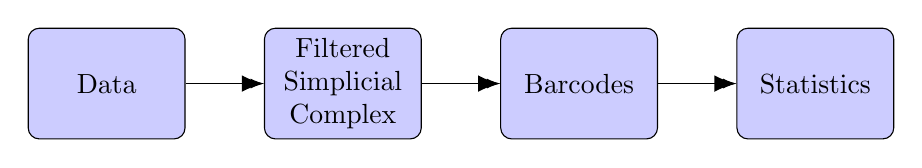
\begin{tikzpicture}[node distance = 2.5cm, auto, scale=0.8, decoration={
      markings,
      mark=at position 1 with {\arrow[scale=2,black]{latex}};
    }
  ]
   % Place nodes
    \node [block] (data) {Data};%Underling Probability Space
    \node [block, right of=data, node distance = 3cm] (simplex) {Filtered Simplicial Complex};
    \node [block, right of=simplex,node distance = 3cm] (pd) {Barcodes};
    \node [block, right of=pd, node distance = 3cm] (stat) {Statistics};
   % Draw edges
    \path [line, postaction={decorate}] (data) -- (simplex);
    \path [line, postaction={decorate}] (simplex) -- (pd);
    \path [line, postaction={decorate}] (pd) -- (stat);
  \end{tikzpicture}
\end{frame}

\begin{frame}
  \frametitle{Overview of PH}
\centering
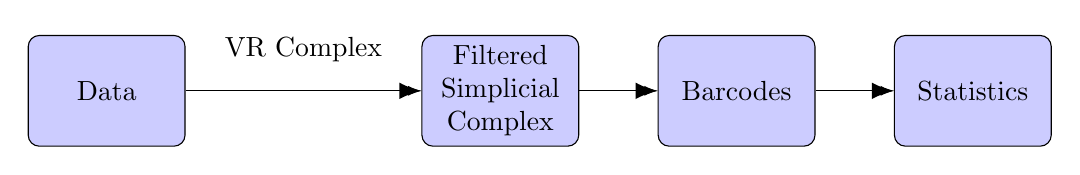
\begin{tikzpicture}[node distance = 2.5cm, auto, scale=0.8, decoration={
      markings, mark=at position 1 with {\arrow[scale=2,black]{latex}};
    }
  ]
   % Place nodes
    \node [block] (data) {Data};
    \node [block, right of=data, node distance = 5cm] (simplex) {Filtered Simplicial Complex};
    \node [block, right of=simplex,node distance = 3cm] (pd) {Barcodes};
    \node [block, right of=pd, node distance = 3cm] (stat) {Statistics};
   % Draw edges
    \path [line, postaction={decorate}] (data) -- (simplex) 
    node [midway, label=above:VR Complex] {};
    \path [line, postaction={decorate}] (simplex) -- (pd);
    \path [line, postaction={decorate}] (pd) -- (stat);
  \end{tikzpicture}
\end{frame}

\begin{frame}
  \frametitle{Simplicial Complexes from Point data}
  \only<1>{\begin{block}{Definition}
    A {\em point cloud} $P$ is a finite metric space.
  \end{block}
}
\only<2->{\begin{block}{Definition}
    The Vietoris-Rips complex is a simplicial complex built out of a point cloud. Put a circle
    of radius $r$ around each point. Add an edge whenever two circles overlap. 
    Add a triangle whenever three circles overlap.
\end{block}
}
  

  \begin{center}
    \only<+>{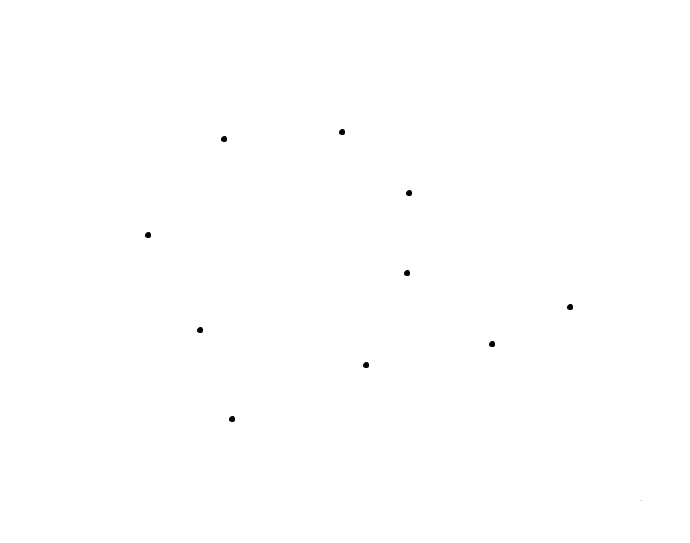
\includegraphics[trim=0 0 0 1cm, clip, scale=0.7]{images/VR_ex_r1.PNG}}
    \only<+>{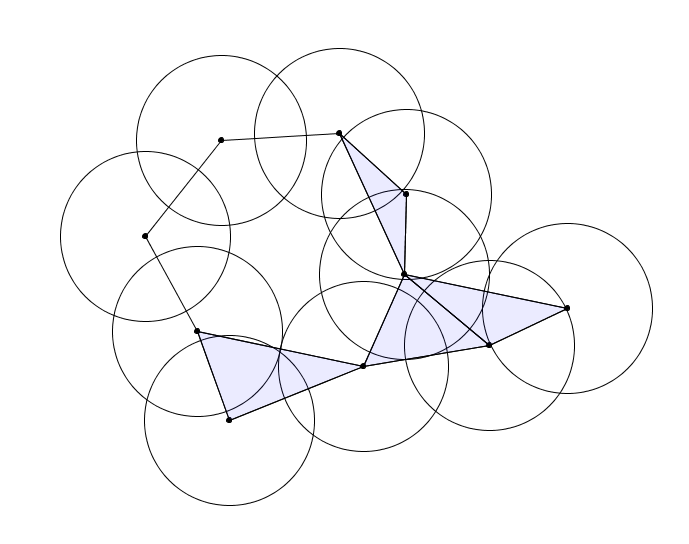
\includegraphics[trim=0 0 0 1cm, clip, scale=0.6]{images/VR_ex_r2.PNG}}
    \only<+>{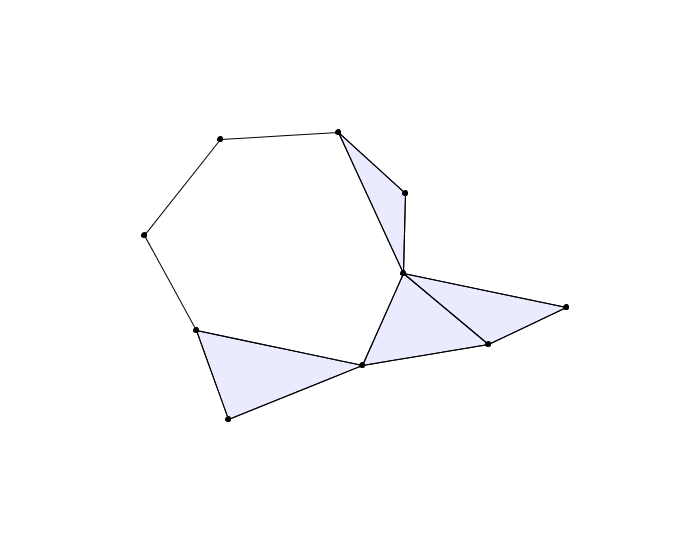
\includegraphics[trim=0 0 0 1cm, clip, scale=0.6]{images/VR_ex_r3.PNG}}
  \end{center}
\end{frame}

\begin{frame}{Vietoris-Rips parameter}
  \begin{block}{Question}
  How do we choose the correct radius for the Vietoris-Rips construction?
\end{block}

Often, there is no one ``right'' choice.
\begin{center}
  \only<+>{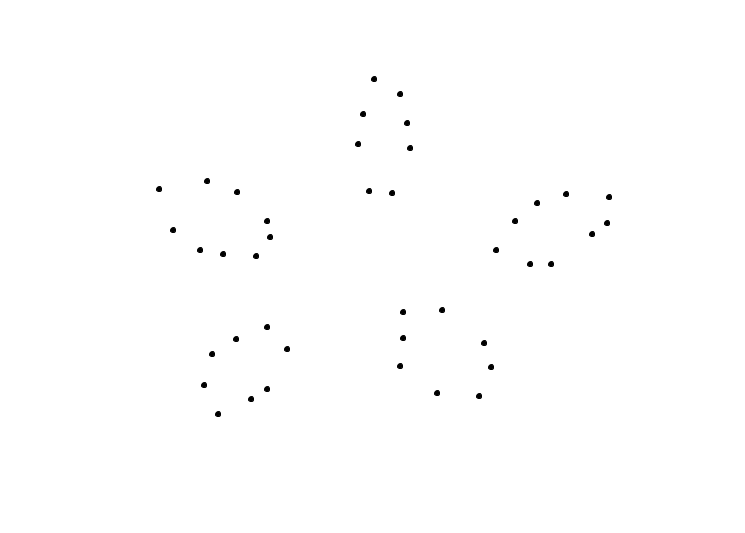
\includegraphics[trim= 0 0 0 1cm, clip, scale=0.7]{images/VR_ex_1.PNG}}
  \only<+>{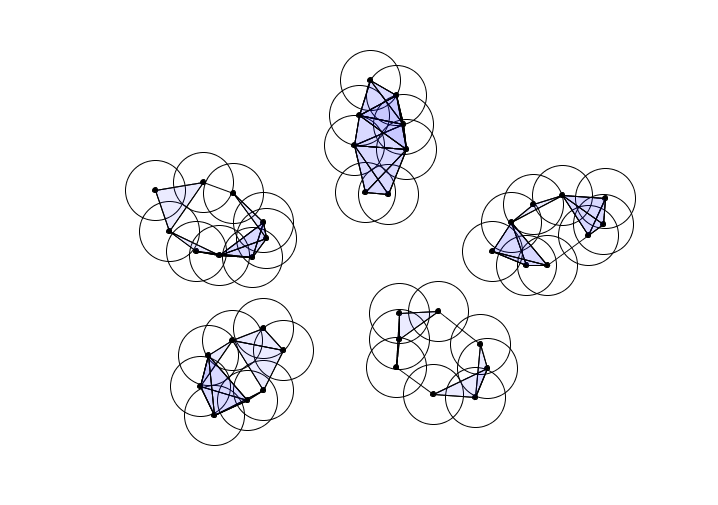
\includegraphics[trim= 0 0 0 1cm, clip, scale=0.7]{images/VR_ex_2.PNG}}
  \only<+>{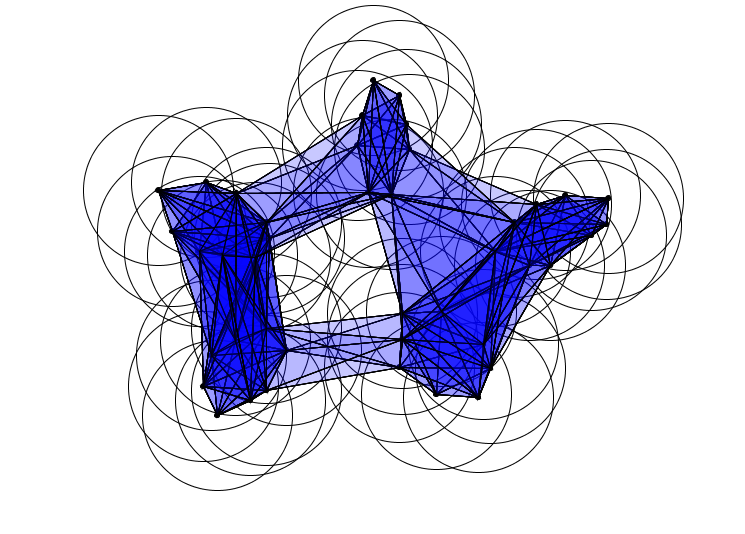
\includegraphics[trim= 0 0 0 1cm, clip, scale=0.7]{images/VR_ex_4.PNG}}
\end{center}
\end{frame}

\begin{frame}{Processing demo}
  \begin{center}
  Processing demo
\end{center}
\end{frame}

\begin{frame}{Overview of PH}
\centering
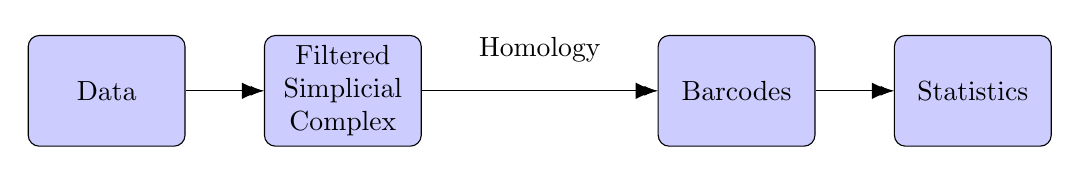
\begin{tikzpicture}[node distance = 2.5cm, auto, scale=0.8, decoration={
      markings,
      mark=at position 1 with {\arrow[scale=2,black]{latex}};
    }
  ]
   % Place nodes
    \node [block] (data) {Data};
    \node [block, right of=data, node distance = 3cm] (simplex) {Filtered Simplicial Complex};
    \node [block, right of=simplex,node distance = 5cm] (pd) {Barcodes};
    \node [block, right of=pd, node distance = 3cm] (stat) {Statistics};
   % Draw edges
    \path [line, postaction={decorate}] (data) -- (simplex);
    \path [line, postaction={decorate}] (simplex) -- (pd)
    node [midway, label=above:Homology] {};
    \path [line, postaction={decorate}] (pd) -- (stat);
  \end{tikzpicture}
\end{frame}

\begin{frame}{Barcodes}
  \begin{itemize}
    \item The barcode provides a summary of how the homology changes as the
      radius varies in the Vietoris-Rips construction.
    \item We look for topological features which `persist' over many values of radii.
  \end{itemize}

  Barcodes typically look like:

  \begin{minipage}{\textwidth}
  \begin{minipage}{0.5\textwidth}
    \centering
    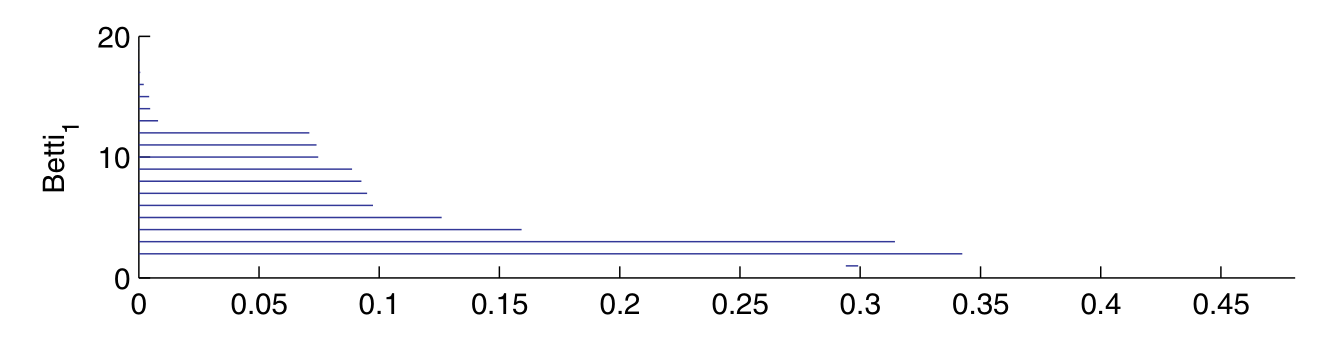
\includegraphics[scale=0.25]{images/betti1.png}
  \end{minipage}
  \begin{minipage}{0.5\textwidth}
    \centering
    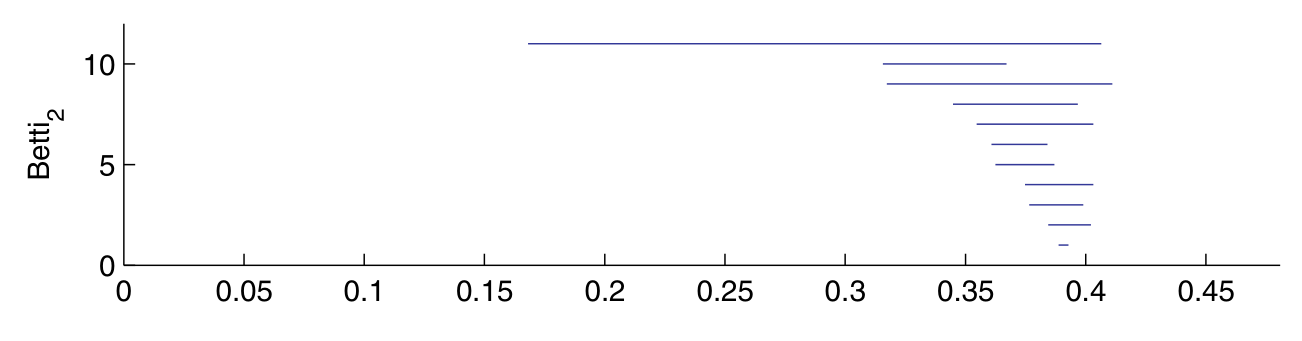
\includegraphics[scale=0.25]{images/betti2.png}
  \end{minipage}
\end{minipage}
\end{frame}

\begin{frame}{Processing demo}
  \begin{center} Processing demo \end{center}
  \end{frame}

\begin{frame}{Overview of PH}
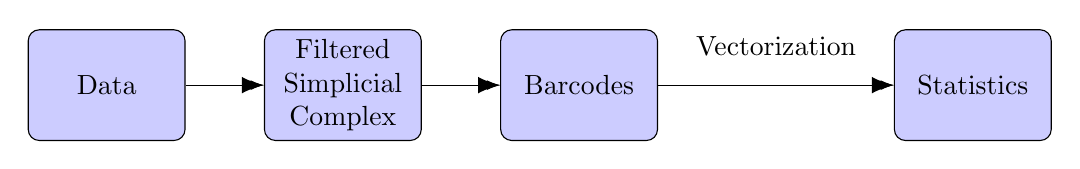
\begin{tikzpicture}[node distance = 2.5cm, auto, scale=0.8, decoration={
      markings,
      mark=at position 1 with {\arrow[scale=2,black]{latex}};
    }
  ]
   % Place nodes
    \node [block] (data) {Data};
    \node [block, right of=data, node distance = 3cm] (simplex) {Filtered Simplicial Complex};
    \node [block, right of=simplex,node distance = 3cm] (pd) {Barcodes};
    \node [block, right of=pd, node distance = 5cm] (stat) {Statistics};
   % Draw edges
    \path [line, postaction={decorate}] (data) -- (simplex);
    \path [line, postaction={decorate}] (simplex) -- (pd);
    \path [line, postaction={decorate}] (pd) -- (stat)
    node [midway, label=above:Vectorization] {};
  \end{tikzpicture}
\end{frame}

\begin{frame}{Vectorization}
  \begin{itemize}
    \item The barcode provides a convenient visualization of persistent topological
      features of potentially high-dimensional data sets. With barcodes:
      \begin{itemize}
	\item Clustering, certain hypothesis testing are {\color{blue} easy},
	\item Calculating averages, understanding variances, and classification are {\color{red}
	  hard}.
	\item {\color{green} Reason:} No good metric space structure on barcodes directly.
      \end{itemize}
    \item We need a way of {\em vectorizing} the output. If we can map the barcodes into
      a vector space, we can add, take differences, averages, etc. 
    \item We can implement more advanced statistical methods, e.g., machine learning
      techniques like SVM.
  \end{itemize}
\end{frame}

\begin{frame}{Persistence Landscapes}
  Relatively simple, yet powerful method of vectorization.
  \begin{minipage}{\textwidth}
    \begin{minipage}{0.7\textwidth}
      \begin{center}
	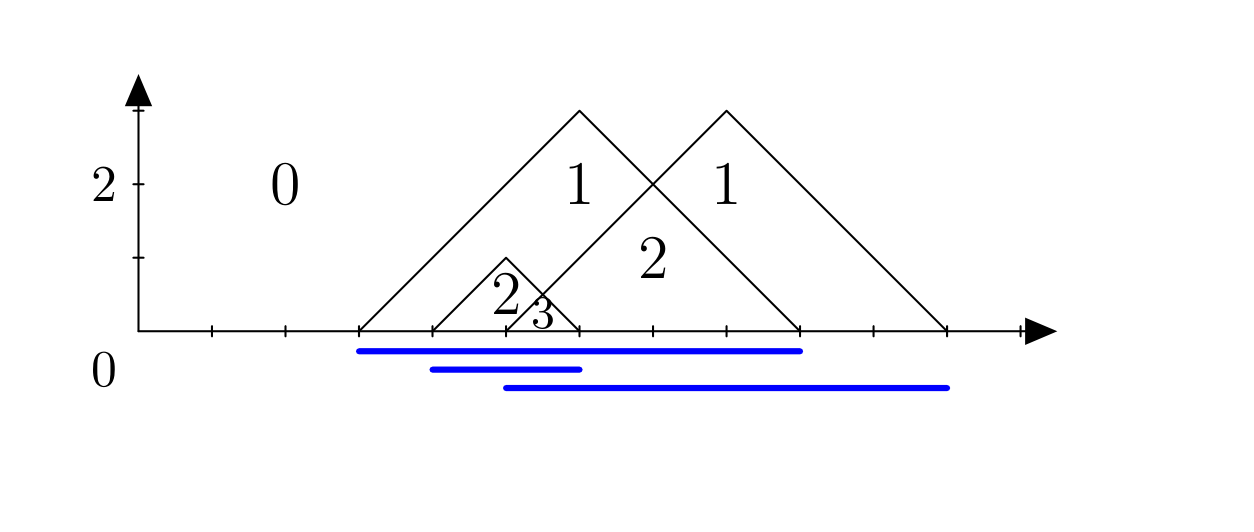
\includegraphics[scale=0.3]{images/l1.png}

	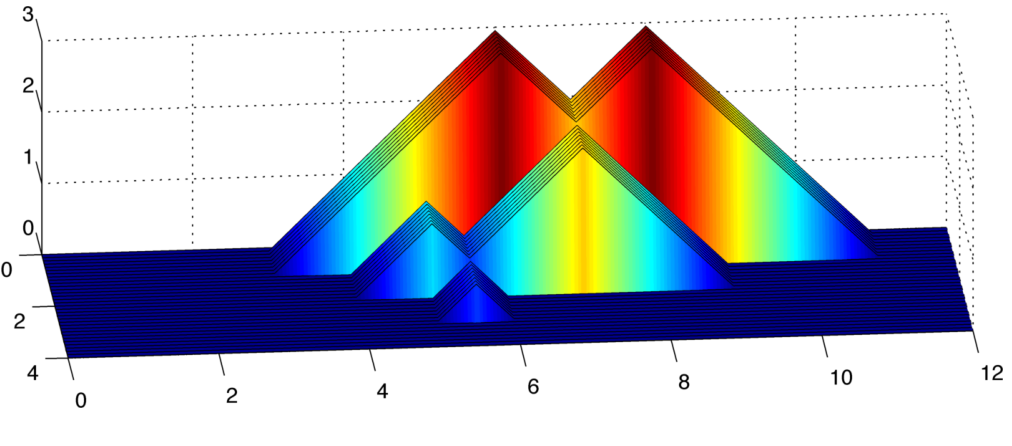
\includegraphics[scale=0.3]{images/l3.png}
      \end{center}
    \end{minipage}
    \begin{minipage}{0.25\textwidth}
      Each 
      \[
	\lambda_k: \R \to \R \, .
      \] 
      Functions can be added, subtracted, averaged, etc.

    \end{minipage}
  \end{minipage}
\end{frame}

\begin{frame}{PH example: mathematical data}
  \begin{itemize}
    \item We sample 1000 points from a noisy sphere and a noisy torus.
      \begin{center}
	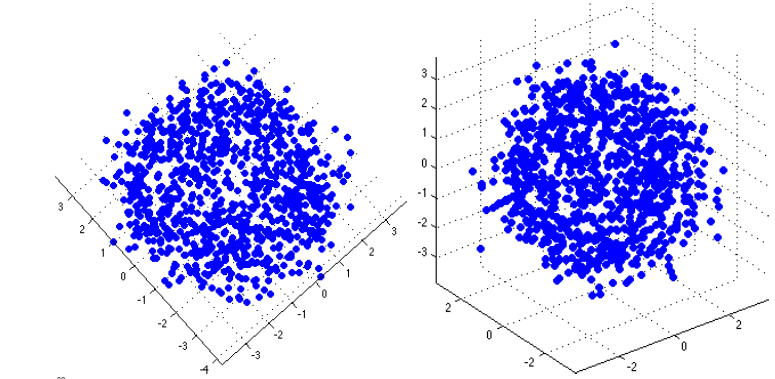
\includegraphics[scale=0.5]{images/sphere_tor.png}
      \end{center}
    \item Can we use persistent homology to distinguish these spaces?
  \end{itemize}
\end{frame}

\begin{frame}{PH example: mathematical data}
  \begin{itemize}
    \item Randomly choose 10 points from each space. Build the VR complex on 
      those 10 points, compute $\beta_0$ barcodes, and build landscapes. 
    \item Repeat this 10,000 times. Average all the sphere landscapes and average
      all the torus landscapes.
      \begin{center}
	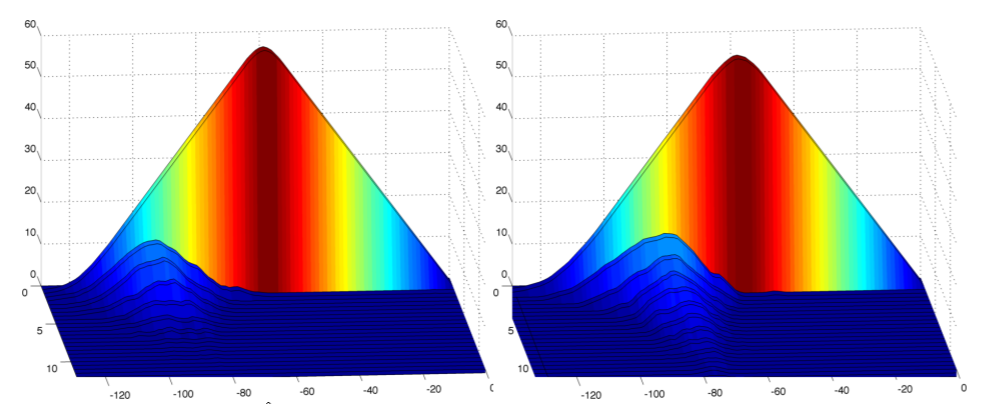
\includegraphics[scale=0.4]{images/pl_compare1.png}
	\pause
	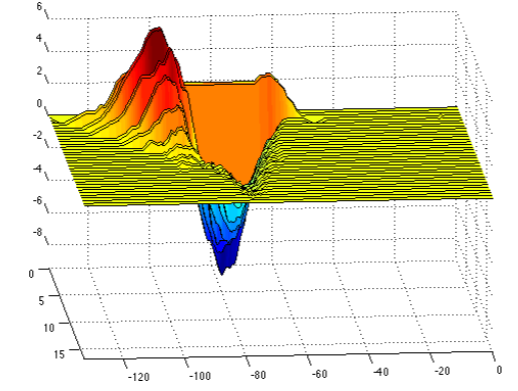
\includegraphics[scale=0.4]{images/pl_comp2.png}
      \end{center}
  \end{itemize}
  Doing a permutation test with 10,000 repetitions gives a p-value of 0.0111!

  {\tiny Peter Bubenik, Statistical Topological Data Analysis using persistence landscapes,
  JoMLR, 2015.}
\end{frame}


\begin{frame}{PH example: fMRI data}
  \begin{itemize}
    \item An fMRI patient has a screen in front of them. They tap
	a pad every time a stimulus flashes on the screen. The stimuli flash both periodically,
	randomly for 200 seconds. There are also rest periods.
      \item We focus on a region of the brain known as the Anterior Cingulate Cortex (ACC).
      \item {\bf Can persistent homology tell the difference between
	these periods based on the fMRI signal?}
  \end{itemize}
\end{frame}

\begin{frame}{PH example: fMRI data}
  \begin{itemize}
    \item The fMRI machine treats the brain as a 3-dimensional grid, so 
      the data is 5-dimensional: $(x,y,z,t,\mathrm{BOLD})$.
    \item For each time slice, compute the VR complex, and then the
      barcodes and landscapes.
    \item Average the periodic time periods, random time periods, and rest time periods.
    \item Doing a permutation test with 10,000 repetitions gives:
  \end{itemize}
  \begin{minipage}{0.7\textwidth}
    \centering
    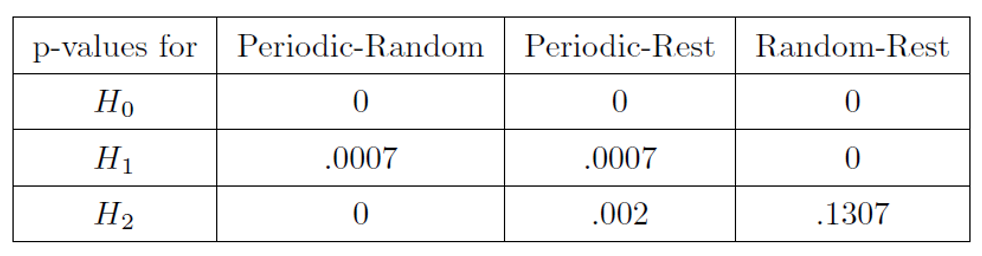
\includegraphics[scale=0.4]{images/ptest.png}
  \end{minipage}
  \begin{minipage}{0.25\textwidth}
    \centering
    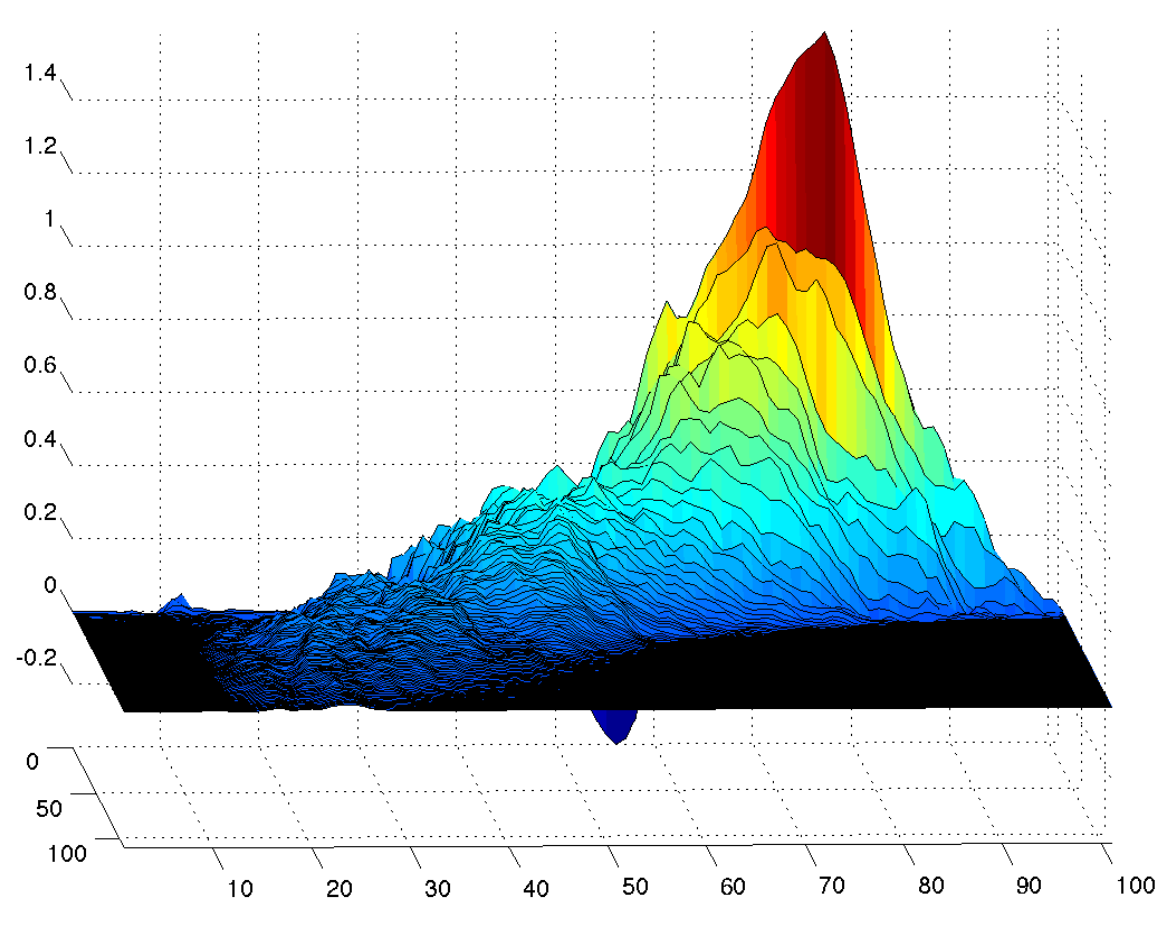
\includegraphics[scale=0.15]{images/pl_h1.png}
  \end{minipage}
\end{frame}

\section{Mapper and examples}
\begin{frame}{Mapper}
  Originally developed by Carlsson and Singh, Mapper provides a different approach
  to classification of data.

  \begin{enumerate}
    \item Choose a `filter' function on the point cloud $f:P \ra \R$.
    \item Cover $\R$ and pull back to cover the point cloud $P$ using $f$.
    \item Within each open set, run single-linkage clustering
    \item Draw a node for each cluster. Connect two nodes from different covers with an edge if they share linked points.
  \end{enumerate}

  \begin{center}
    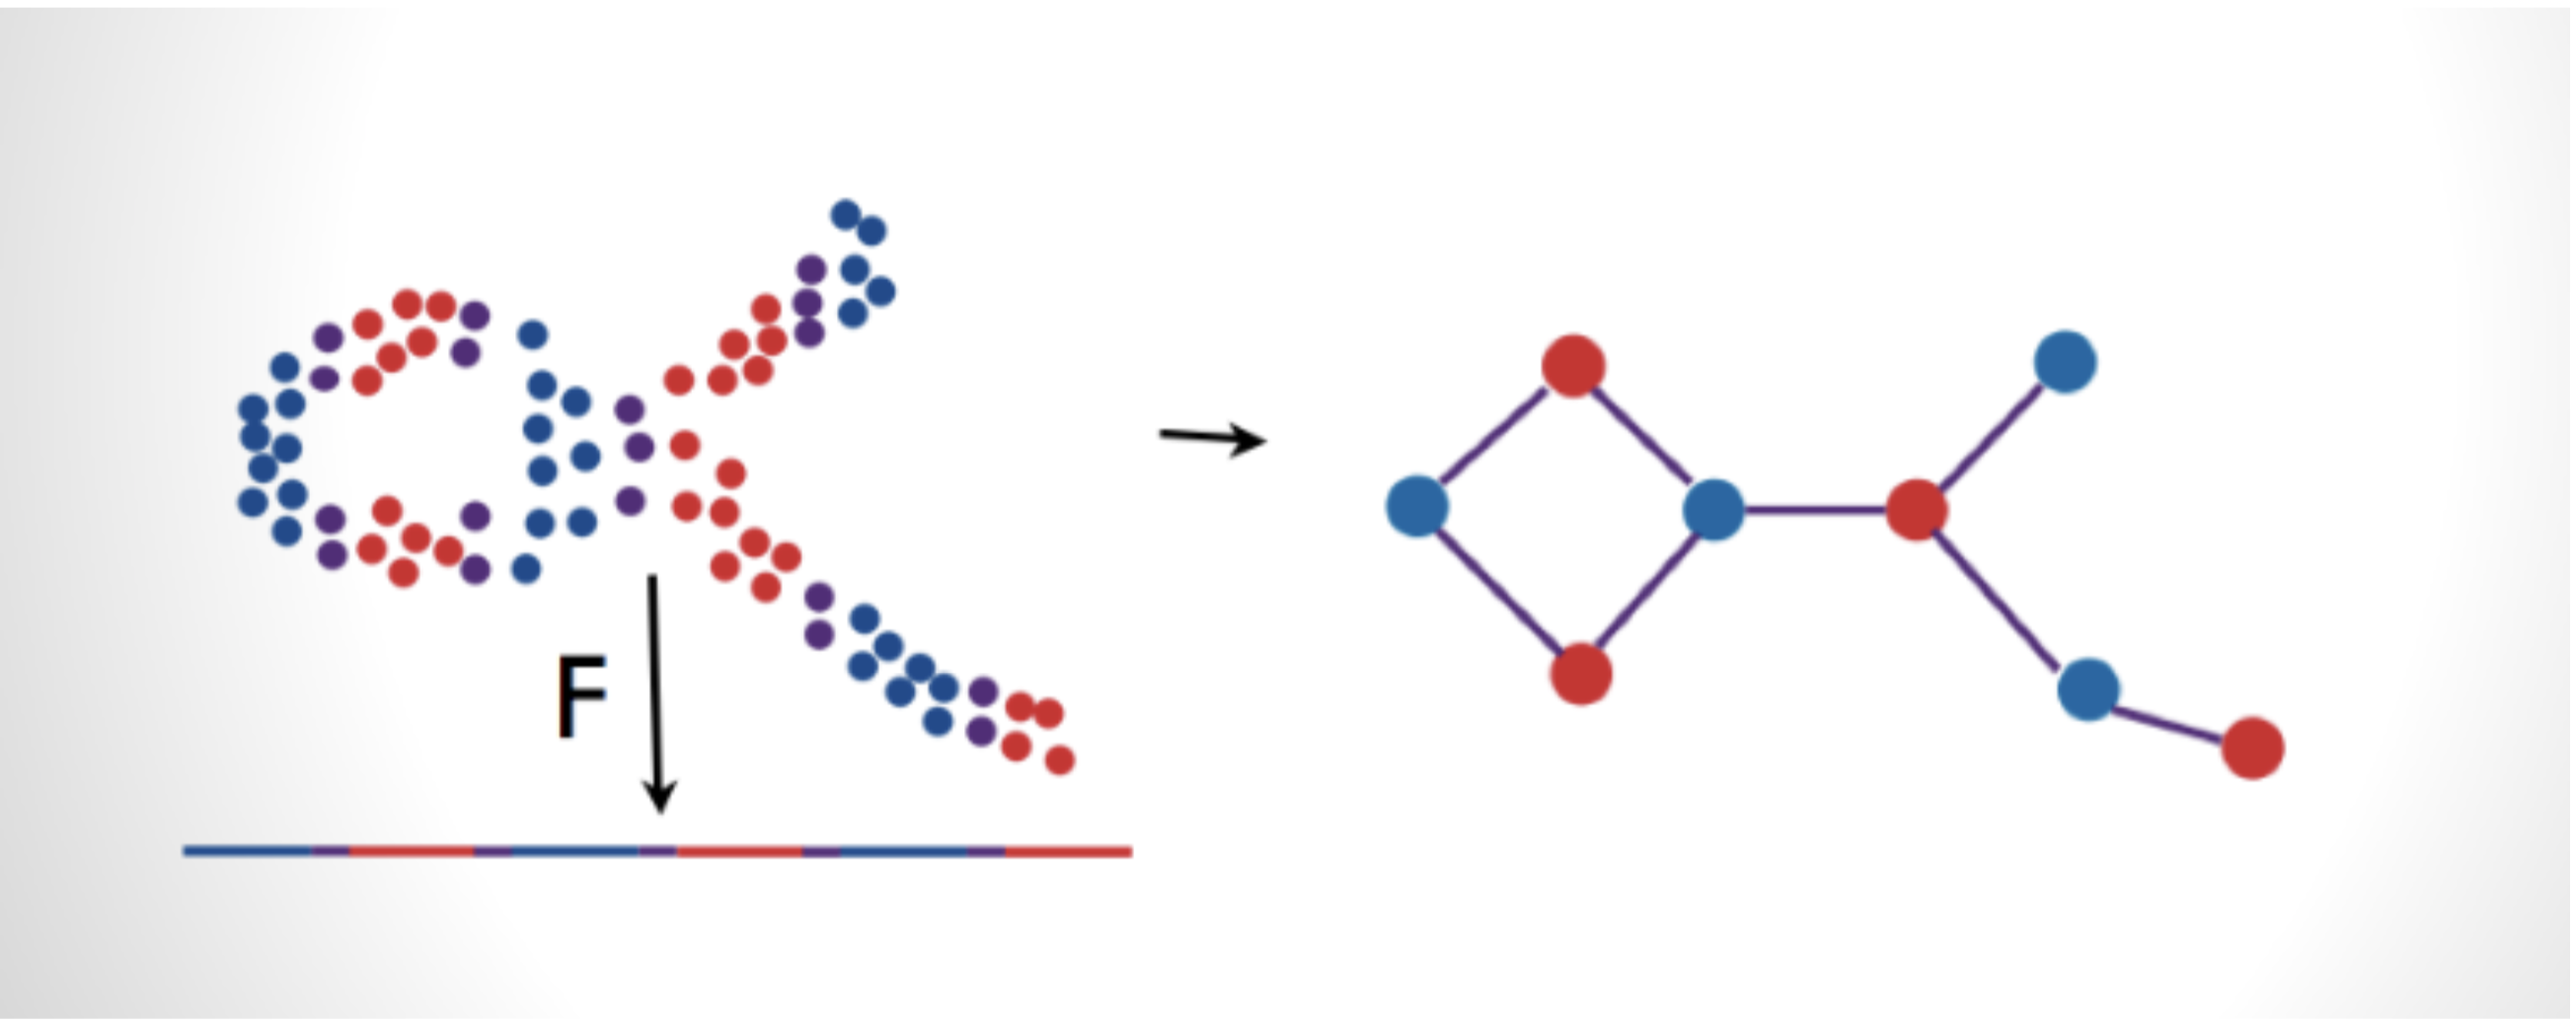
\includegraphics[scale=0.2]{images/mapper1.png}
  \end{center}
\end{frame}

\begin{frame}{Mapper properties}
 \begin{itemize}
   \item Mapper provides a different form of visualization of high dimensional
     data compared to persistent homology.
   \item Complimentary method to persistent homology, as well other 
     statistical methods.
   \item There are several parameters to be chosen. In particular, 
     the {\color{red} filter function $f$} needs to be chosen carefully!
 \end{itemize}

 \begin{center}
   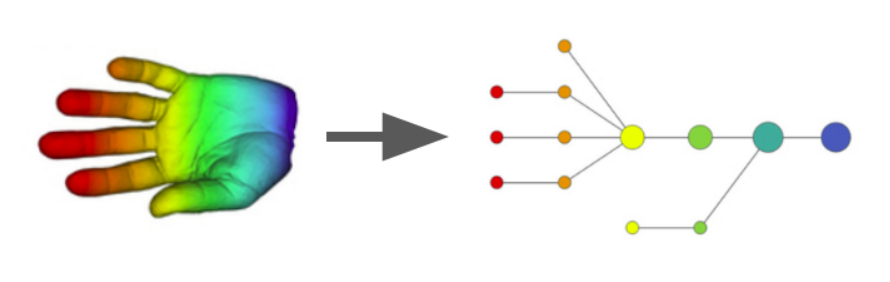
\includegraphics[scale=0.5]{images/mapper_hand.png}
 \end{center}
 \end{frame}

 \begin{frame}{Mapper examples: Breast cancer}
   \centering
   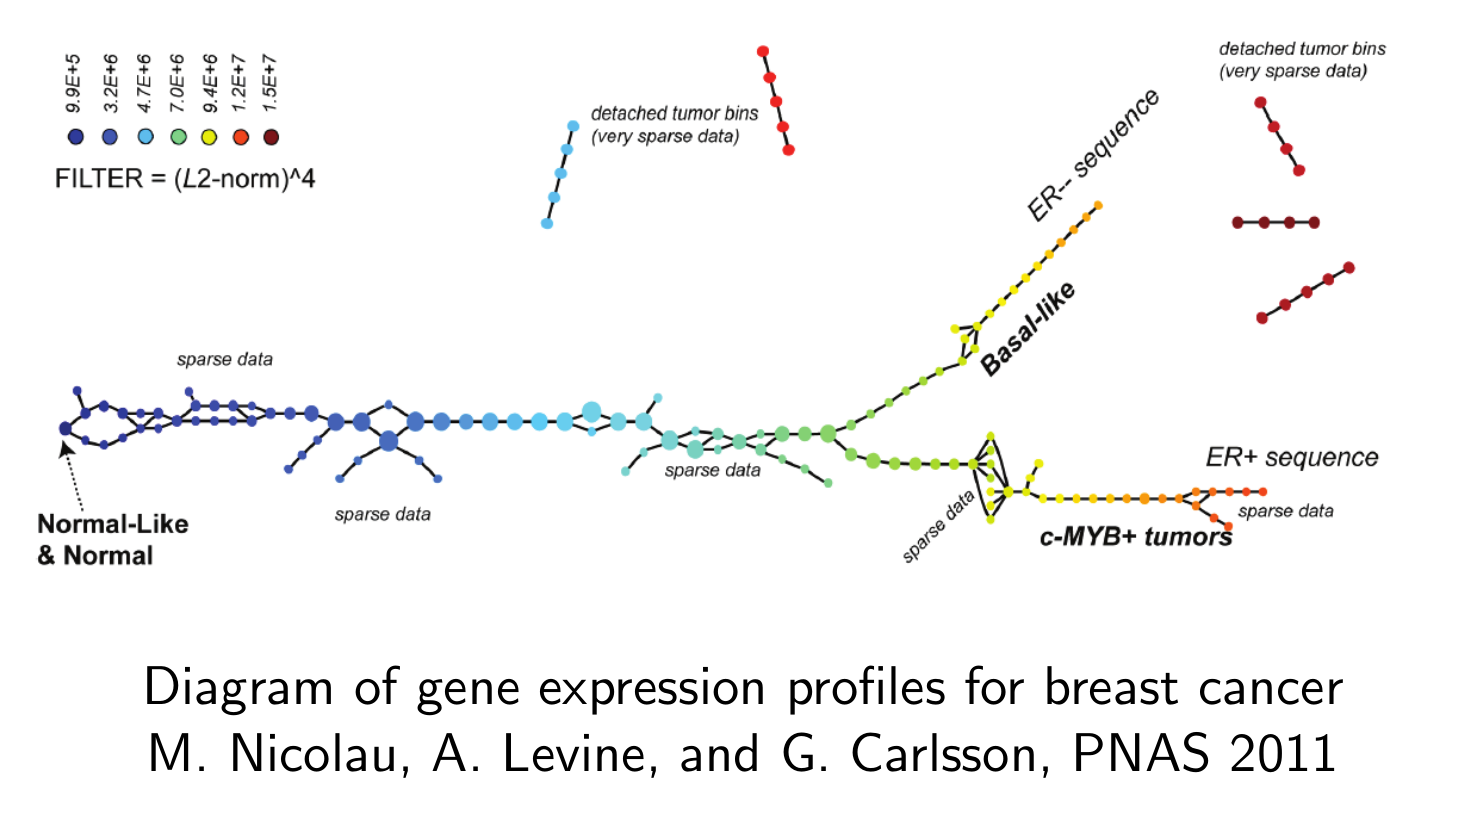
\includegraphics[scale=0.4]{images/mapper_cancer.png}
 \end{frame}

 \section{Implementation and resources}
\begin{frame}{Algorithms}
  There are lots of software packages implementing the algorithms of persistent homology:

  \begin{minipage}{0.4\textwidth}
    \centering
    \underline{Persistent Homology:}
  \begin{itemize}
      \begin{multicols}{2}
    \item Javaplex
    \item Dionysus
    \item Perseus
    \item {\color{red} Ripser}
    \item PHAT
    \item GUDHI
    \item CHOMP
    \item SimBa
    \item SimPers
    \item Eirene
    \item R-TDA
    \end{multicols}
  \end{itemize}
\end{minipage}
  \begin{minipage}{0.3\textwidth}
    \centering
    \underline{Vectorizations:}
  \begin{itemize}
    \item Persistence landscapes
    \item Persistence images
    \item Persistence silhouettes
  \end{itemize}
\end{minipage}
\begin{minipage}{0.25\textwidth}
  \centering
  \underline{Mapper:}
  \begin{itemize}
    \item Pymapper
    \item TDAmapper
  \end{itemize}
\end{minipage}
\end{frame}

  %\nocite{ghrist2017homological, carlsson_topology_2009, perea_brief_2018, wright}


\begin{frame}{References}
\nocite{ghrist2017homological, bubenik_statistical_2015, carlsson_topology_2009,
oudot2015persistence, perea_brief_2018, wright}

\renewcommand*{\bibfont}{\small}
General Overviews:
\printbibliography[keyword=intro]

More technical introduction:
\printbibliography[keyword=nintro]

%  \nocite{bubenik_statistical_2015,oudot2015persistence}

%  \printbibliography[title={More technical Overviews}]
\end{frame}


\end{document}
